\chapter{Theoretical Background}\label{chp:theory}

\section{Literature Review}\label{sec:litreview}

The literature review in \Cref{sec:litreview} presents past and present research on utilisation of machine learning methods to achieve energy efficient operation. The concept of different modelling approaches for ship operation will be discussed in \Cref{sec:modelling_type}. Short summary of the data source in the modelling of FOC is given in \Cref{sec:data_use}. The review of popular machine learning model used to predict FOC is presented in \Cref{sec:ml_var_appl}. The performance of tree-based model, which include random forest and extra trees in various research will be discussed in \Cref{sec:tree_litreview}. Brief summary of the literature review is presented in \Cref{sec:lit_review_conclusion}.\\

\subsection{Modelling Approach for Ship Operation}\label{sec:modelling_type}

According to \bcitet{MichaelHaranen.2016} and \bcitet{Coraddu.2017}, the modelling strategies to predict fuel consumption are classified into three categories:\\

\subsubsection*{\textbf{White Box Models (WBM)}} Based on \emph{a priori} mechanistic knowledge and physical principles of the vessel's system. This means that the dimensions of the vessel's structure, design parameters, and propulsion plant configuration are known.\\

\subsubsection*{\textbf{Black Box Models (BBM)}} Purely data driven, and it is developed using data from different sailing journey and historical observations. Contrary to WBM, this approach does not require detailed information on the vessel. This modelling approach can be further split into two categories. \emph{Statistical Modelling} aims to find explanations for relationships between fuel consumption and different factors that affect it. \emph{Machine Learning (ML) Modelling} focuses on the predictive capabilities of the model that could predict fuel consumption at different points in time.\\

\subsubsection*{\textbf{Grey Box Models (GBM)}} Fuse WBM and BBM into a single model that considers both \emph{a priori} knowledge of the vessel and historical sailing data, This method aims to complement the performance of WBM and BBM.\\

Each of these strategies possesses its strength and limitations. WBMs are developed based on physical and hydrodynamics laws as well as theories of naval architecture, it is transparent and comprehensible, making them the preferred model used by various shipping industries. However, the deterministic nature of WBMs causes them to have poor suitability and generalisability. This is mainly caused due to limited \emph{a priori} knowledge of different vessel dimensions, parameters, and narrow application limits of principle dimensions and form parameters of the vessel. Subsequently, the inability of WBMs to add randomness makes it rigid and restrictive. \bcitep{MichaelHaranen.2016,Yan.2021}\\

BBMs in general have a good fitting ability for training data and good predictive accuracy for unseen data. BBMs developed using machine learning approach can generalise better compared to BBMs that are based on statistical modelling \bcitep{Petersen.2012b}. BBMs are purely data driven, which means BBMs do not require former knowledge of vessel principle dimensions and form parameters. With increasing amount of data, better generalisation performance and handling of noisy data should be expected in a BBM. However, for the same reason, the quality of BBM model is highly dependent on data quantity and quality. For BBMs based machine learning approach, the amount of data is a major factor in determining the effectiveness of machine learning \bcitep{Halevy.2009}. Data driven approach means that BBMs neglect basic vessel physical knowledge and are generally complex making it challenging to analyse and explain. For these reasons, experts in shipping industries are critical of models that do not include basic vessel knowledge and those that violate concepts of the domain knowledge in serious ways \bcitep{Yan.2021}.\\   

Hence, GBMs are introduced to address the limitations of both WBMs and BBMs by combining the mechanistic knowledge of the ship and physical principles of the vessel's system with BBM models, which possess good predictive capability. Despite these advantages, \bcitet{Yan.2021} noted that GBM approach is not a common approach, recent research to predict fuel consumption are mainly dominated by BBM approach, specifically BBM based on machine learning approach.\\

\subsection{Review of data source used for FOC model}\label{sec:data_use}

The modelling of FOC using GBM requires both components of WBM and BBM. For the BBM modelling part using machine learning approach, it is especially important to ensure sufficient amount of good quality data to be available for model training to ensure precise and accurate training of the model \bcitep{Halevy.2009}. It summarised by \bcitet{Yan.2021}, that the modelling of FOC use the following types of data source:\\

\subsubsection*{\textbf{(Daily) Noon Report}} Daily reports manually filed by ship's chief engineer and sent by the ship's masters to the shipping company and shore management. The reports include informations on types of daily fuel consumption, basic voyage information (e.g. ship location, load condition), sailing behaviour information e.g. (average sailing speed, average engine revolution per minute (RPM)), as well as sea and weather conditions. While it provides relevant information regarding the ship operation, the inherent problem of daily and manual data entry means that the quality and quantity of data cannot be guaranteed.\\

\subsubsection*{\textbf{Sensor Data}} Data obtained from installed sensor onboard the vessel. This may include fuel flow sensors, Global Positioning System (GPS) receiver and wind speed sensors are among the possible sensors that can be installed onboard a vessel. Sensor data address the issues of data quantity from noon report, as pointed out in the study by \bcitet{Gkerekos.2019} for the prediction of daily FOC. The machine learning models, which are produced by the Automated Data Logging and Monitoring (ADLM) system outperforms the models that used noon data for their training by $5-7\%$ for a collection period of 3 months of the ADLM system and 2.5 years for the noon data. However, installing onboard sensors may be complex and costly \bcitep{JoanPeturPetersen.2011} and the resulting sensor data will need to be handled properly to account for error in the sensors.\\

\subsubsection*{\textbf{AIS Data}} Apart from its intended use as collision avoidance system, AIS data have seen potential usage in ship behaviour analysis and environmental analysis. The Green House Gas (GHG) study by IMO \bcitep{IMO.2020,T.W.P.Smith.2015}, uses AIS to estimate global shipping emission inventories. \bcitet{Rakke2016} proposed a methodology termed ECAIS to calculate ship emissions based on the fuel consumption from AIS data. Through Holtrop-Mennen approximation and literature approximation, the ship's power propulsion can be determined which is subsequently used to predict specific fuel consumption. \bcitet{Kim.2020b} used publicly accessible AIS data, ship static data, and environmental data to estimate EEOI using big data technology. Generally, the study using AIS data is done to achieve independence from the need to use commercial databases. The details of AIS data will be discussed in \Cref{sec:ais_theo}\\  

\subsection{Review of ML approach to predict FOC}\label{sec:ml_var_appl}

Modelling of FOC using \emph{machine learning} approach generally focus on prediction of unseen data. The general framework usually include collection and preprocessing of ship operational data, training and validation of the model, and evaluation and selection of the most appropriate model. Some machine learning models allow further hyperparameter tuning of the model and in case of data rich environment, the data can be further split into test data to further validate the performance of machine learning model.\\

The study by \bcitet{Yan.2021} indicated that the majority of recent research that uses machine learning approach employ ANN as the model to predict FOC. ANN models are powerful models capable of modelling nonlinear data which are based on theories on how the brain works. The outcome is modelled by intermediate set of unobserved variables known as hidden layer. \bcitep{Kuhn.2013}. Back propagation neural networks, Multi Level Perceptron (MLP), and wavelet neural networks are some examples of ANN model subclasses.\\

ANN has shown respectable performance in its attempt to predict FOC. \bcitet{Petersen.2012} reported Root Mean Square Error of $47.2$ L/h for the fuel flow i.e. FOC. To put this into context, the fuel flow in their case study fluctuates between $1000 - 2500$ L/h. \bcitet{BalBesikci.2016} considered sailing speed, trim, wind, sea effects, propeller pitch, and engine rotation speed as input variables to predict FOC per hour and achieved model fit score of $R^2 = 0.759$ in test set. Other studies also reported similar range of results using ANNs \bcitep{Yan.2021}.\\

However, the development of ANN models is a challenging task. ANN models tend to overfit when there is shortage of data, as such, regularisation is necessary to improve model performance. The balancing process during regularisation is a demanding task and unsuitable regularisation may lead to counterintuitive prediction results. Adding layers is computationally expensive, and it does not always guarantee promising results \bcitep{Hastie.2009}. Additionally, in machine learning terms, ANN is classified as a black box model, which makes it unintuitive and lacking in interpretability  \bcitep{Geron.2019}, this particular limitation cause shipping industry expert generally reluctant to accept the model generated using machine learning approach. \\

\subsection{Tree-Based Model as FOC model}\label{sec:tree_litreview}

Concerning interpretability, modelling approaches such Linear Regression (LR), KNN and tree-based models have shown superior interpretability in comparison to ANNs. LR can explain the effect of each input variable on the output through the coefficients. KNN searches for the nearest neighbour and their closeness is evaluated through distance measurement algorithms such as Euclidean distance. Additionally, LRs and KNNs also offer easy implementation and adequate explainability. However, both approaches suffer from sensitivity to outliers and noise in data.\\

This brings us to tree-based model, a supervised, highly interpretable machine learning modelling approach capable of performing classification tasks for discrete data and regression tasks for continuous data. According to summary of \bcitet{Yan.2021}, it is not as popular as ANN, however some literature work and studies have indicated its benefits and performance superiority over other machine learning modelling approaches:\\

\bcitet{Soner.2018} used the ferry dataset from \bcitet{Petersen.2012} to predict FOC using tree-based model, which includes bagging, random forest (RF), and bootstrap. From the test dataset, the random forest model achieved RMSE of $43.5$ L/h for the fuel consumption. Which suggested improvement from ANN model from the study of \bcitet{Petersen.2012}.\\ 

\bcitet{Yan.2020} used random forest (RF) model to predict FOC for a voyage of a dry bulk ship using ship operational data i.e. ship noon data and sea and weather data from noon report and EMCWF. The prediction model considered ship sailing speed, total cargo weight and meteorological conditions and  RF model obtained mean absolute percentage error (MAPE) of $7.91\%$ for the FOC. The RF model displayed superior result in comparison to Decision Tree Regressor (DTR), ANN, LASSO, and SVR.\\      

The advantage of tree-based model is further highlighted by \bcitet{Gkerekos.2019}. The study compared the performance of different machine learning models to predict ship's FOC per day using both noon data and automated data logging and monitoring (ADLM) system from a bulk carrier. This research concludes that tree-based model displayed good prediction performance on both noon data and sensor-based data. ETR achieved remarkable model fit score of $89\%$ using the noon data and $97\%$ when using the data from ADLM system, outperforming ANN, SVR, and RFR models.\\

\bcitet{Li.2022} performed more extensive research on the effects of data fusions between meteorological data, ship voyage data, and AIS data on different machine learning models to predict the ship's FOC. The study classified ETR and RFR as tree-based model which is produced by \emph{bagging ensemble strategy}. While AdaBoost (AB), Gradient Tree Boosting (GB), XGBoost(XG) and LightGBM (LB) are classified as tree-based models produced by \emph{boosting ensemble strategy}. The study recommends all tree-based models that are produced by \emph{boosting ensemble strategy} and ETR to be used to model energy efficient operation. Additionally, RFR shows the best robustness among the proposed model in the study.\\

\bcitet{Abebe.2020} attempted to use machine learning approach to predict SOG of the ship. In this study, AIS data and noon-report weather data from 14 tracks and 62 ships are used for model training. The model considered the ship draught, ship dynamic information, tonnage, and environmental conditions. The result of this study exhibited the feasibility of using AIS data and meteorological data to predict SOG of the ship. The results also further indicated the strength of tree-based model, on test dataset, ETR achieved the best result with model fit of $98.47\%$ and RMSE of $0,234$ knots. It is also reported that ETR achieved better performance with about half of the computational cost of RFR.\\ 

\subsection{Review of WBM for FOC prediction}\label{sec:wbm_review}

To predict the FOC of a ship, WBMs usually calculate the resistances encountered by the vessel based on physics and hydrodynamic laws. The total resistance is summed from resistance of calm water resistances and additional resistance from wind, wave, and other external factors. The corresponding engine power at a particular speed can be calculated, and consequently the FOC can be calculated.\bcitep{MichaelHaranen.2016}\\

The methods from \bcitet{Guldhammer.1974}, \bcitet{Hollenbach.1999}, and \bcitet{Kristensen.2012} use different formulations, assumptions, and input variables for engine power estimation. For this thesis, the main focus will be the use of the estimation method from Holtrop-Mennen \bcitep{Holtrop.1978,Holtrop.1982,Holtrop.1984}. Holtrop-Mennen estimate method allowable application range is suitable in most of the cases. This is indicated by studies from \bcitet{Rakke2016} and \bcitet{Kim.2020b}. \bcitet{Rakke2016} used ship operational and mechanical data from various works of literature and AIS data for input variables to estimate the engine power using Holtrop-Mennen method to subsequently calculate FOC. The FOC is then used to estimate GHG emissions for different ships and the study reported about $5\%$ error rate during model testing. \bcitet{Kim.2020b} successfully estimated Energy Efficiency Operational Index (EEOI) without actual FOC. The study used AIS data as well as publicly accessible weather data and ship static information. The approach in this study used Holtrop-Mennen method to estimate engine power which is consequently used to calculate FOC for EEOI estimations.\\ 

\subsection{Conclusion of Literature Review}\label{sec:lit_review_conclusion}

As termed by \bcitet{Yan.2021}, the GBM model in this thesis falls under the category of sequential GBM, where the BBM and the WBM will be developed in series and combined to form a single GBM. The BBM will be developed to perform initial prediction and the resulting prediction will be passed into the WBM. The use of tree-based regressor, which will be used to predict SOG, provides solution to the problem of poor interpretability of some machine learning models. Furthermore, tree-based models can outperform most of the available machine learning models while providing added benefits of little requirement for data preprocessing and relatively cheap computational cost. The selection of Holtrop-Mennen as engine power estimation method is justified by the application range of the methodology and successes from previous studies.\\ 

\section{Tree-based model}\label{sec:tree_intro}

Decision Tree, Random Forest and Extra-Tree are classified as tree-based model, which is supervised machine learning model capable of classification tasks for discrete variables and regression tasks for continuous variables. In this section, the theory of Decision Tree (DT), Random Forest (RF) and Extra Tree (ET) will be discussed in detail in \Cref{sec:dt_theo}, \Cref{sec:rf_theo} and \Cref{sec:et_theo}.\\  

\subsection{Decision Tree}\label{sec:dt_theo}

The principle of decision tree as a predictor can be defined as one or more nested {\tt if-then} statements based on a rule that partitions the data into partition space as shown in \Cref{fig:partitionspace}. Alternatively, the partition space generated from {\tt if-then} statements can be represented using binary tree representation, which is more interpretable as multiple input response can be represented by a single tree.\bcitep{Kuhn.2013,Hastie.2009}\\ 

A decision tree consists of the following type of nodes, \textbf{\emph{Root node}} defines the topmost node. \textbf{\emph{Leaf nodes}} are also termed as terminal nodes, it is the node that will give the final prediction output. The
\textbf{\emph{Internal Node}} is defined as the nodes between the root node and leaf node. The process of dividing a node into successive nodes is called \textbf{\emph{splitting}}. The node that is being split is called \textbf{\emph{parent node}} and the successive nodes that are created are called \textbf{\emph{child nodes}}. To grow a tree in a regression task, the splitting process is commonly regulated by Mean Square Error (MSE). The tree growth algorithm are based on Classification and Regression Tree (CART).\\

To understand the principle of selection for the feature, $k_t$ , of the parent node and splitting rule, $t_k$ , for data partition, the following example will be presented:\\

\begin{figure}
\centering
\begin{minipage}[b]{.5\textwidth}
    \centering
    \begin{tikzpicture}[x=0.75pt,y=0.75pt,yscale=-1,xscale=1]
    %uncomment if require: \path (0,433); %set diagram left start at 0, and has height of 433
    
    %Shape: Square [id:dp5731268858272198] 
    \draw   (180,110) -- (370,110) -- (370,300) -- (180,300) -- cycle ;
    %Straight Lines [id:da615072570759449] 
    \draw    (250,110) -- (250,300) ;
    %Straight Lines [id:da8002566967918264] 
    \draw    (300,110) -- (300,300) ;
    %Straight Lines [id:da4409034763483005] 
    \draw    (180,230) -- (250,230) ;
    %Straight Lines [id:da07514682530914596] 
    \draw    (300,170) -- (370,170) ;
    
    % Text Node
    \draw (131,192.4) node [anchor=north west][inner sep=0.75pt]    {$X_{2}$};
    % Text Node
    \draw (261,340.4) node [anchor=north west][inner sep=0.75pt]    {$X_{1}$};
    % Text Node
    \draw (157,222.4) node [anchor=north west][inner sep=0.75pt]    {$t_{2}$};
    % Text Node
    \draw (201,252.4) node [anchor=north west][inner sep=0.75pt]    {$R_{1}$};
    % Text Node
    \draw (201,162.4) node [anchor=north west][inner sep=0.75pt]    {$R_{2}$};
    % Text Node
    \draw (268,192.4) node [anchor=north west][inner sep=0.75pt]    {$R_{3}$};
    % Text Node
    \draw (321,132.4) node [anchor=north west][inner sep=0.75pt]    {$R_{4}$};
    % Text Node
    \draw (321,220.4) node [anchor=north west][inner sep=0.75pt]    {$R_{5}$};
    % Text Node
    \draw (241,310.4) node [anchor=north west][inner sep=0.75pt]    {$t_{1}$};
    % Text Node
    \draw (291,312.4) node [anchor=north west][inner sep=0.75pt]    {$t_{3}$};
    % Text Node
    \draw (381,162.4) node [anchor=north west][inner sep=0.75pt]    {$t_{4}$};
    
    \end{tikzpicture}
    
    \captionof{figure}{Example of partition space \bcitep{Hastie.2009}} 
    \label{fig:partitionspace}
\end{minipage}%
\begin{minipage}[b]{.5\textwidth}
    \centering
    \begin{tikzpicture}
        \tikzset{level distance=65pt,sibling distance=10pt,edge from parent/.style=
        {draw,edge from parent path={(\tikzparentnode.south)
                                -- +(0,-8pt)
                                -| (\tikzchildnode)}}}
    \Tree [.$X_1\leq t_1$ [.$X_2\leq t_2$ [.$R_1$ ] [.$R_2$ ] ]
        [.$X_1\leq t_3$ [.$R_3$ ]
        [.$X_2\leq t_4$ [.$R_4$ ] [.$R_5$ ] ] ] ]
    \end{tikzpicture}
    \captionof{figure}{Example of partition tree \bcitep{Hastie.2009}} 
    \label{fig:partitiontree}
\end{minipage}
\end{figure}

\textbf{For the selection of the optimal splitting rule $t_k$}: Given a case with single feature $k$ and response $y$ with $m$ data points present. The algorithm starts by looking for possible splits between two distinct data points $y$. This split results in two distinct partition spaces. For each partition space $S_1$ and $S_2$, the mean is calculated by dividing the sum of response $y$ with the amount of data points $m$ for each respective partition space $S_1$ and $S_2$.\\ 

This step is then followed by calculating the sum of squared error (SSE) of each data point in partition space $S_1$ and $S_2$ and dividing it by the number of data points $m_{s_1}$ and $m_{s_2}$ respectively to obtain the MSE. Subsequently, the MSE from the respective partition space $S_1$ and $S_2$ is summed. The process is then recursively repeated until a threshold $t_k$ that produces minimum sum of MSE is found, this threshold will be selected as splitting rule for the parent node and correspond to the threshold that minimise the cost function $J(k,t_k)$, with $\hat{y}_{S_i}$, being the mean of the response, $y_{S_i}$, in partition space $S_i$. \bcitep{Geron.2019,Kuhn.2013}:

\begin{equation}\label{eqn:sse}
    \text{MSE}_{S_i} = \frac{1}{m_{S_i}}\text{SSE}_{S_i} \quad \textbf{where} \quad i = (1,2)   
\end{equation}
\begin{equation}\label{eqn:costfun}
    J(k,t_k) = \frac{1}{m_{S_1}}\text{SSE}_{S_1} + \frac{1}{m_{S_2}}\text{SSE}_{S_2}
    \begin{cases}
        \text{SSE}_{S_i} = \sum\limits_{i \in S_i}(\hat{y}_{S_i} - y_{S_i} )^2 \\
        \hat{y}_{S_i} = \frac{1}{m_{S_i}}\sum\limits_{i\in S_i} y
    \end{cases}  
\end{equation}

\textbf{For the selection of the most optimal feature for parent node $t_k$}: Similar principle is also applied for the selection of the most optimal feature for the parent node. Consider there are $k_t$ features, then for each respective feature $k_1,k_2,\dots,k_t$, The MSE for each of the features is calculated following the cost function $J(k,t_k)$. The feature that can best \emph{\textbf{minimise}} the cost function will be selected as the root node of the tree. The subsequent selections of the feature for the parent node follow the same principle. \bcitep{Hastie.2009,Geron.2019}.\\

Once complete, then the partition space is further split into two more regions to look for the next possible split that minimise the cost function $J(k,t_k)$. This process is recursively continued until the number of samples to split falls under a certain threshold or when it cannot find a split that can further reduce MSE.\\ 


\begin{figure}[h]
    \centering
    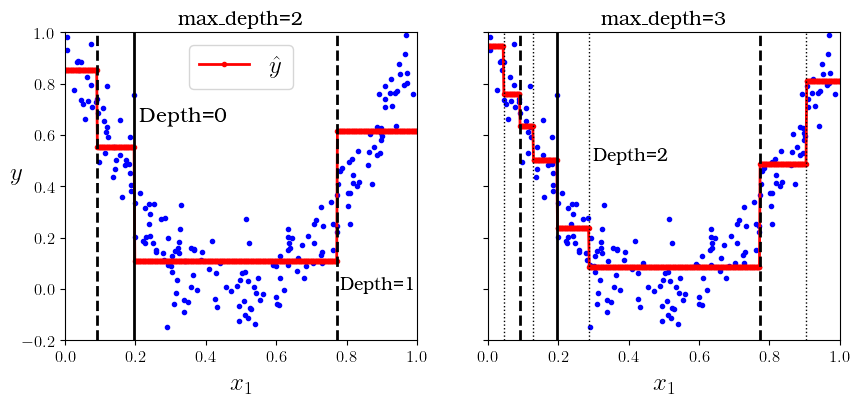
\includegraphics[width=.9\textwidth]{02_figures/fig6_5_partspace_geron09.png}
    \caption{Prediction of two Decision tree regression models \bcitep{Geron.2019}}
    \label{fig:geron6_5}
\end{figure}

The resulting decisions for the best possible splits can be represented using binary tree, this makes decision tree highly interpretable and easy to implement. The inherent logic structure from {\tt if-then} statements means that it can handle various types of data (sparse, skewed, continuous, categorical, etc.) without the need for data pre-processing. Decision tree implicitly conducts feature selection which is a desirable trait for many modelling problems \bcitep{Kuhn.2013}.\\

However, a single decision tree suffers from overfitting when the model is unconstrained. The logical principle of {\tt if-then} statements means that decision tree will attempt to fit the training data as closely as possible. Furthermore, a single decision tree model tends to be unstable, altering the data will cause drastic changes in the structure of the tree, there exist possibilities where completely different sets of splits might be found resulting in different interpretations \bcitep{Hastie.2009,Kuhn.2013}.\\

From \Cref{fig:partitionspace}, it can be implied that each decision boundaries are orthogonal to an axis i.e. all splits are perpendicular to an axis and this form rectangular subspaces for each predicted value. If the relationship between predictors and response cannot be adequately defined by the rectangular subspaces, then tree based models will suffer from larger prediction error than other kinds of models \bcitep{Kuhn.2013}.\\

Therefore, it is necessary to regularise i.e., restrict the decision tree's freedom to grow during model training. Overfitting could be reduced by controlling how deep the tree can grow through the {\tt max\_depth} parameter. Additionally, setting the amount of minimum number of samples a leaf node has, through {\tt min\_samples\_leaf} can alleviate overfitting as well, as shown in \Cref{fig:geron6_6}. Other regularisation techniques will be discussed in \Cref{sec:hpo}.\\ 

Regularisation of decision tree will help to address the overfitting issues and improve the robustness of the model, this may result in better generalisation capability. Nonetheless, in order to attain significant improvements in the performance of decision tree model, it is necessary to seek alternative solutions.\\

\begin{figure}
    \centering
        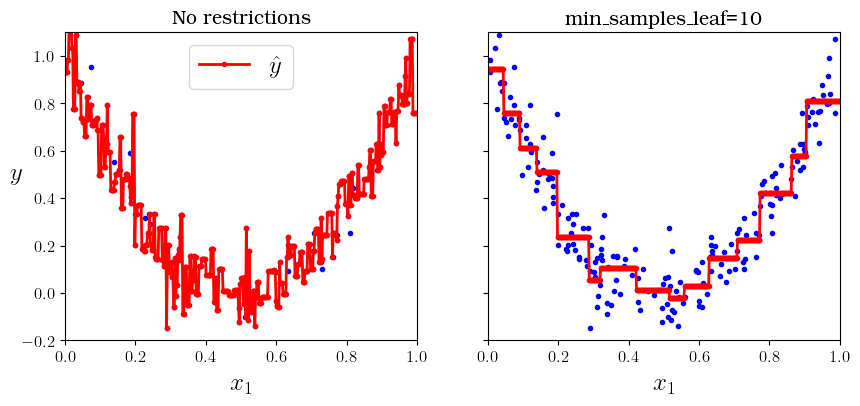
\includegraphics[width=.9\textwidth]{02_figures/fig6_6_paramdepth_geron09.png}
        \caption{Regularising a Decision Tree regressor \bcitep{Geron.2019}}
        \label{fig:geron6_6}
\end{figure}

\subsection{Random Forest}\label{sec:rf_theo}

Ensemble learning is one of the possible solutions to improve the performance of DT regressors. The main idea of ensemble learning is combining the strengths of a collection of simpler base models \bcitep{Hastie.2009}. The algorithm, involving the creation of bootstrap samples, random selection of splitting feature and aggregation of the prediction is termed by \bcitet{Breiman.2001} as \textbf{\emph{Random Forest}}. It involves combination of multiple learning algorithms, known as weak learners. In random forest, each of these learners are individual decision tree.\\

The most common ensemble methods are \emph{boosting} and \emph{bagging}. In boosting, the learner evolves over time, where successive trees are dependent on the earlier trees. In bagging (short for \emph{bootstrap aggregating}) each tree is trained using bootstrap sample of the training set i.e. this means that a sample of the training dataset is randomly selected and allowed to appear more than once\footnote{This sampling technique is referred to as sampling \emph{with} replacement}. Each model in the ensemble then generates a prediction from the bootstrapped sample and the predictions are aggregated across the learners \bcitep{TinKamHo.1995,Breiman.2001}.\\

The performance of bagging can be further improved by reducing correlation between trees i.e. de-correlating trees. This can be achieved by adding randomness during tree construction process. \bcitet{Dietterich.2000} introduced the idea of random split selection, which means that a feature $k$ will be selected from a random subset of feature. From this random subset, the assignment of the feature for the parent node follows the CART algorithm described in \Cref{eqn:costfun}. Further randomness is added by exploiting the instability of single decision tree mentioned in \Cref{sec:dt_theo}.\\

The methodology introduced in random forest address the tendency of decision tree to overfit and the issue of lack of robustness. De-correlating trees means that each learner is independent of each other, and the combination of many independent, strong learners yields an improvement in error rates i.e. reduction in variance and robustness against noisy response. It is also proven by \bcitet{Breiman.2001} that random forest cannot overfit, that means growing more trees should not affect the performance of random forest, albeit with a greater computational burden. Both \bcitet{Kuhn.2013} and \bcitet{Hastie.2009} reported that remarkable prediction results can be obtained without extensive tuning of tree parameter. \\

However, random forest loses the benefit of interpretability of tree-based model. Due to ensemble nature of random forest, it is not possible to gain an understanding between the feature and the prediction. Nevertheless, it is still possible to quantify the impact of each feature in the ensemble \bcitep{Kuhn.2013}\footnote{Known as feature importances in \scikit/}. Random forest also tends to perform poorly with small number of samples \bcitep{Hastie.2009}. Nevertheless, it is possible to traverse through a single tree to see the path taken to reach the predicted value.\\

\subsection{Extra-Trees (Extremely Randomised Trees)}\label{sec:et_theo}

Extra-trees (Extremely Randomised Trees) is introduced by \bcitet{Geurts.2006} to further randomise random forest and further de-correlate the trees in the forest. Unlike random forest, which selects the optimal split by selecting the best feature among randomly selected subset of features, Extra-trees selects a split at random. Extra-trees also does not bootstrap the sample\footnote{This sampling technique is referred to as sampling \emph{without} replacement} and uses the whole training dataset. The random selection of split means that it saves computational power and the increase in variance caused by tree de-correlation can be countered by increasing the number of trees in the ensemble.\\ 

\section{AIS Data}\label{sec:ais_theo}

\subsection{Overview of AIS}

Automatic Identification System (AIS) is an automated tracking system onboard ships to automatically transmit information about the ship to other ships and coastal authorities, AIS was developed to avoid ship collision accidents. As part of the revised new chapter V of SOLAS\footnote{International Convention for the Safety of Lives at Sea} regulation, International Maritime Organization (IMO) requires all international voyage ships of 300 gross tonnage (GT) and upwards, cargo ships with 500 GT not engaged on international voyage, and all passenger ships irrespective of size to be equipped of AIS class A equipment \bcitep{Yang.2019,webimo.2014}.\\

AIS uses Very High Frequency (VHF) with special protocol for communication system for information exchange between the ships. This information will be received by either ships directly, buoys, Land based AIS transceivers (T-AIS) and satellites (S-AIS). The information transmitted by AIS is distinguished into three different types. \textbf{Static information} which is entered into the AIS on installation. \textbf{Dynamic information}, which is automatically updated from the ship's sensors connected to AIS and \textbf{voyage-related information}, which might need to be manually entered and updated during the voyage. The structure of the AIS data that is relevant to this thesis is summarised in \Cref{tbl:AIS_struct}\bcitep{webimo.2014}.\\

AIS is also further differentiated by its equipment class. The classification is based on the reporting interval and the type of information that is conveyed. \textbf{Class A} autonomously report their position within 2-10 seconds interval, depending on the state of ship's movement. The reporting interval is less frequent at 3 minutes, When the ship is at anchor or moored and moving slower than 3 knots. Class A AIS is also capable of sending safety related information, meteorological and hydrological data, electronic broadcast to mariners and marine safety messages. \textbf{Class B} reports at longer interval and at a lower power. They can only receive safety related messages, not send them. \bcitep{Rakke2016,webimo.2014}\\

\begin{table}
    \footnotesize
    \centering
    % \resizebox {\textwidth}{!}
    {\begin{tabular}{ p{0.25\linewidth} p{0.7\linewidth}  }
    \hline
    \textbf{Information Item} & \textbf{Description} \\
    \hline
    \multicolumn{2}{l}{\textbf{Static}}\\
    \hline
    MMSI & MMSI number of vessel\\
    Callsign & Callsign of vessel \\
    Name & Name of the vessel \\
    IMO & IMO number of the vessel \\
    Length & Length of vessel \\
    Width & Width of vessel \\
    Ship Type & Describes the AIS ship type of this vessel \\
    \hline
    \multicolumn{2}{l}{\textbf{Dynamic}}\\
    \hline
    Ship's position & Automatically updated from position sensor connected to AIS. Longitude and Latitude.\\
    Position time stamp in UTC & Automatically updated from ship's main position sensor. Format: DD\slash MM\slash YYYY HH:MM:SS\\
    Course over Ground (COG) & \emph{\textbf{If available}}, automatically updated from ship's main position sensor connected to AIS.\\  
    Speed Over Ground (SOG) & \emph{\textbf{If available}}, automatically updated from the position sensor connected to AIS.\\
    Heading & Automatically updated from the ship's heading sensor connected to AIS\\
    Navigational status & Navigational status information has to be manually entered by the Officer on Watch (OOW) and changed as necessary. For example : ``\emph{underway by engines}'',``\emph{engaged in fishing}'',``\emph{at anchor}''.\\
    Rate of Turn (ROT) & \emph{\textbf{If available}}, Automatically updated from the ship's ROT sensor or derived from
    the gyro.\\
    \hline
    \multicolumn{2}{l}{\textbf{Voyage Related}}\\
    \hline
    Ship's draught & To be manually entered at the start of the voyage using the
    maximum draft for the voyage and amended as required \\
    (Hazardous) Cargo Type & Type of cargo from AIS message.\\
    Destination and ETA & To be manually entered at the start of the voyage and kept up to
    date as necessary.\\
    \hline
    \end{tabular}}
\caption{Structure of AIS data \bcitep{webimo.2014}}\label{tbl:AIS_struct}
\end{table}

It is also stated by \bcitet{Yang.2019} that AIS data can be combined with data from other databases to provide additional information such as:\\

\begin{itemize}
    \setlength\itemsep{0em}
    \item Port to port average speed, the voyage time can be calculated from the time stamps reported by AIS data; the voyage distance can be found from corresponding navigation distance tables.
    \item Cargo weight which can be estimated from draught and ship size.
    \item Technical ship specification from fleet database which can be derived from IMO number.
    \item Port to port bunker consumption which can be estimated based on the speed, technical ship specification and distance between two ports.
\end{itemize}

\subsection{Speed Correction}\label{sec:SOG_corr}

The speed that is shown in AIS is the speed over ground (SOG). However, the ship actual speed i.e. speed through water (STW) will be required to calculate the bunker fuel consumption. Therefore, the SOG will need to be corrected for STW. This correction is performed by considering the current speed $V_c$ and the direction of the current $\gamma$ \emph{with respect to True North}. In principle, STW will be greater than SOG, when the current is moving against the current as the ship tries to compensate for the current to maintain the SOG. Whereas, the STW will be greater than the SOG when the current is moving in the same direction of the ship movement. \\

To calculate the correction, this study will adopt the methodology proposed by Kim et al. \bcitep{Kim.2020b} and Yang et al. \bcitep{Yang.2020}. The $x$ and $y$ component of SOG can be obtained through vector decomposition using the ship's heading angle $\alpha$ \emph{with respect to True North}. Similar vector decomposition is also performed for current speed $V_{\text{current}}$, it is resolved with current direction $\gamma$ \emph{with respect to True North}:\\

\begin{equation}\label{eqn:sogx}
    V_{\text{SOG}}^x = V_{\text{SOG}}\cdot\sin(\alpha)   
\end{equation}
\begin{equation}\label{eqn:sogy}
    V_{\text{SOG}}^y = V_{\text{SOG}}\cdot\cos(\alpha)   
\end{equation} 
\begin{equation}\label{eqn:vcurrx}
     V_{\text{current}}^x = V_{\text{current}}\cdot\sin(\gamma)   
\end{equation}
\begin{equation}\label{eqn:vcurry}
    V_{\text{current}}^y = V_{\text{current}}\cdot\cos(\gamma)   
\end{equation}
Then the resulting equation to determine STW, including the current compensation, is given by:\\
\begin{equation}\label{eqn:stwx}
    V_{\text{STW}}^x = V_{\text{SOG}}^x - V_{\text{current}}^x    
\end{equation}
\begin{equation}\label{eqn:stwy}
    V_{\text{STW}}^y = V_{\text{SOG}}^y - V_{\text{current}}^y      
\end{equation}
\begin{equation}\label{eqn:stwabs}
    V_{\text{STW}} = \sqrt{(V_{\text{STW}}^x)^2 + (V_{\text{STW}}^y)^2} 
\end{equation}

\subsection{Source of error in AIS}\label{sec:AIS_error}

Errors and inaccuracies may still exist in AIS data. The main source of errors is caused by data that requires manual entry such as static information and voyage related information which include estimated time of arrival (ETA) and draught. There exist cases where MMSI is shared by different ships even though it is supposed to be unique. The data that is automatically connected by sensors can be erroneous, this may happen when the sensors are faulty or when it is not properly installed \bcitep{Yang.2019}. Therefore, data preprocessing of AIS data is an important step to ensure correct representation of the ship state.\\    

\section{Weather data}\label{sec:weather_theo}

During voyage, a vessel may encounter winds and waves from different directions with varying degree of magnitude. This may affect the vessel's path taken during the voyage and also ship performance such as speed and engine power, furthermore it may also affect the seakeeping capability of a vessel \bcitep{Molland.2011}. It is important to consider different weather conditions to ensure accurate and precise estimation of required engine power by the vessel. With that in mind, the discussion in this section will focus on definition of wind and wave effects, as well as the relation between some of these parameters. \\  

\subsection{Definitions of weather parameters}\label{sec:weather_definition}

\subsubsection*{Wind Waves and Swell}

\textbf{Wind Waves} are also known as wind sea, wind waves are irregular and short-crested waves generated by local wind. \textbf{Swell} are waves that travel outside the wave generation area and are no longer the result of wind, they take on regular and long-crested appearance \bcitep{Holthuijsen.2007}

\subsubsection*{Significant Wave Height, $H_{1/3}$}

It is defined as the mean of the highest one-third of waves in the wave record. The distribution of wave heights can be represented by probability density function. Hence, the term ``highest one-third of waves'' here means the region of wave heights that belong in the upper one-third of a probability density function, this is illustrated in \Cref{fig:wavestats}. From this distribution, the relation between significant wave height $H_{1/3}$, the highest ten percent of waves $H_{10}$, maximum wave height $H_{max}$ and average wave height $\overline{H}$ can be summarised as follows \bcitep{bretschneider.1965,Holthuijsen.2007}: 
\begin{equation}\label{eqn:Hsig_mean}
    \overline{H} = 0.625\cdot H_{1/3}
\end{equation}
\begin{equation}\label{eqn:Hsig_Hten}
    H_{10} = 2.03\cdot \overline{H} = 1.27\cdot H_{1/3} 
\end{equation}
\begin{equation}\label{eqn:Hsig_max}
    H_{\text{max}} = 2 \cdot H_{1/3} 
\end{equation} 

Additionally, \bcitet{BitnerGregersen.2005} and \bcitet{Nielsen.2020} described the relation between the significant wave height, wind wave height and swell height through following equation:

\begin{equation}\label{eqn:H_sig_root}
    H_{1/3} = \sqrt{(H_{\text{swell}})^2 + (H_{\text{windwave}})^2} 
\end{equation}

\begin{figure}[h]
    \centering
        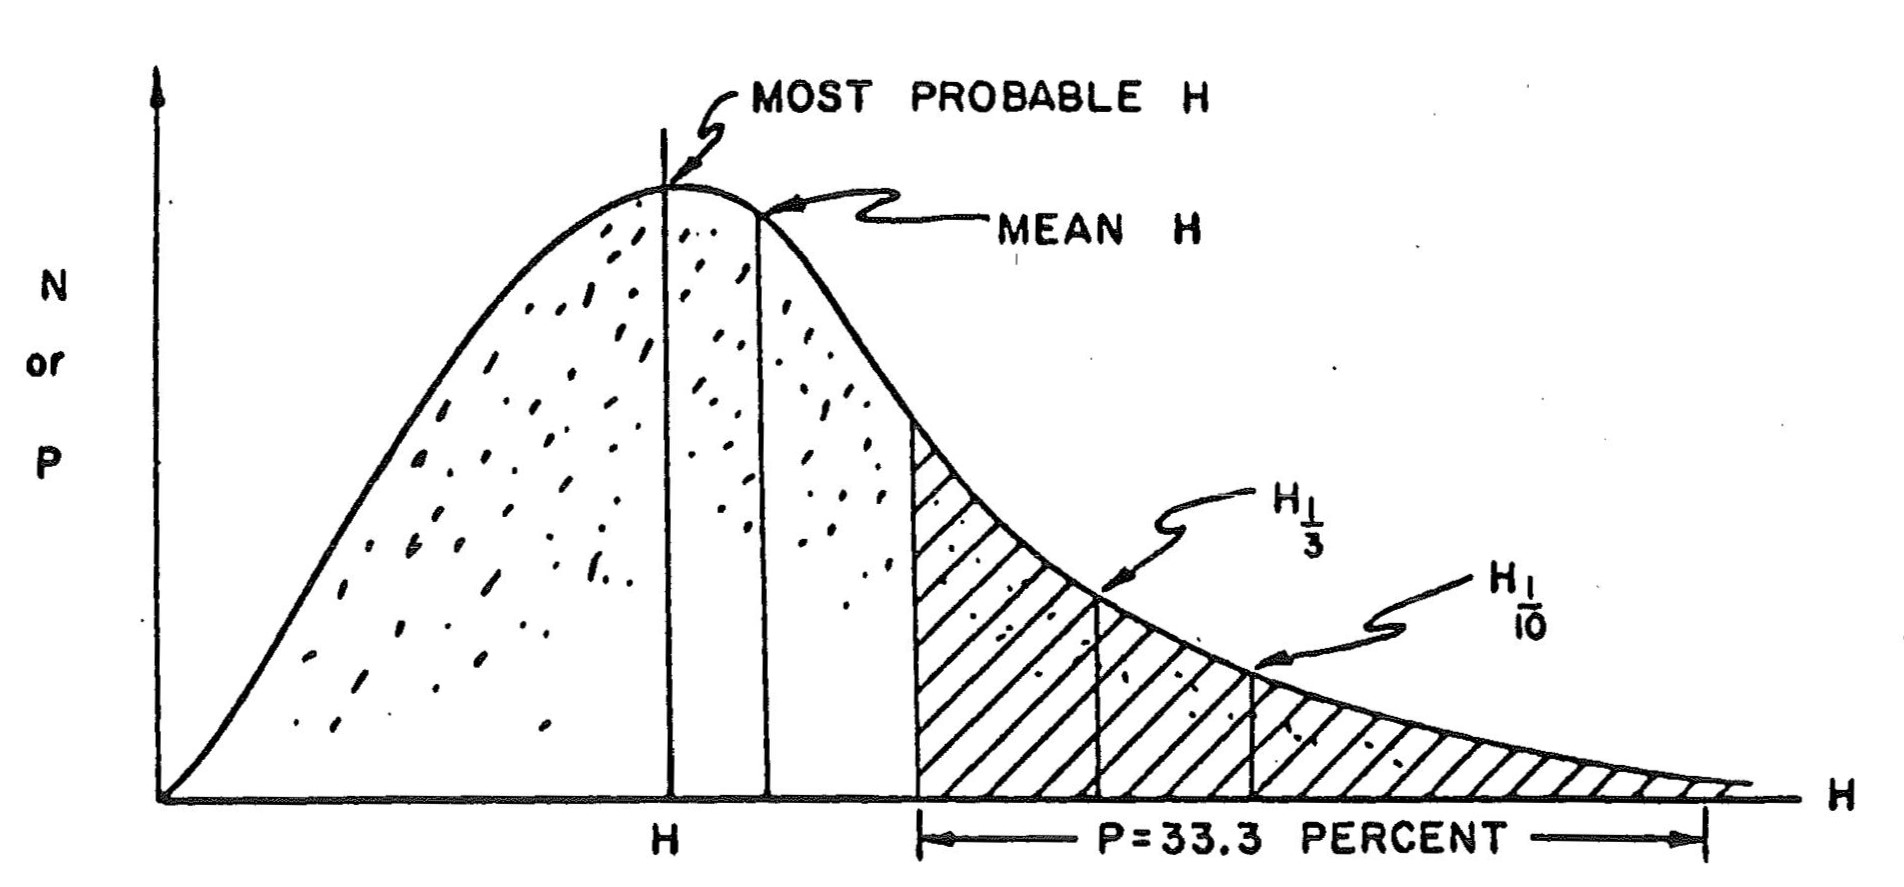
\includegraphics[width=.75\textwidth]{02_figures/Bretschneider_1965_wavedist.jpg}
        \caption{Statistical distribution of wave heights \bcitep{bretschneider.1965}}
        \label{fig:wavestats}
\end{figure}

\subsubsection*{Wave Period}

Defined as the time interval between the start and the end of a wave. Some characteristics of wave period can be derived to define wave spectrum.

\subsubsection*{Wave Spectrum}

The most important form in which ocean waves are described. Wave spectrum characterises all possible observations of the waves which include wave heights, frequencies i.e. period and wave direction. For example, \bcitet{BitnerGregersen.2005} stated that the state of the sea can be described through the significant height $H_{1/3}$ and spectral peak $T_p$ with the help of Torsethaugen peak, given average wave spectrum $T_f$ and constant $a_f = 6.6$  \bcitep{K.Torsethaugen.2004}. 

\begin{equation}\label{eqn:T_p_spectralpeak}
    T_p = a_f\cdot H_{1/3}
\end{equation}
\begin{equation}\label{eqn:currdir}
    \text{Sea State (SS)} = 
    \begin{cases}
        \text{Swell dominated} \quad \text{\textbf{if}} \quad T_p > T_f \\ 
        \text{Wind sea dominated} \quad \text{\textbf{if}} \quad T_p \leqslant T_f \\   
    \end{cases}   
\end{equation}

\section{General concept of ship propulsion}\label{sec:power_calc}

A ship's bunker fuel consumption in actual operating conditions are affected by several factors including the operating parameter of the ship's engine, propeller efficiency and encountered resistance by the ship. Furthermore, a ship's propulsion power is correlated to the sailing speed (SOG) and meteorological conditions \bcitep{XiaoLang.2020}. Therefore, in addition to the calm water resistance $R_{CALM}$, the additional resistance caused by wind $R_{WIND}$ and wave $R_{AW}$ should be considered to estimate the total resistance of the ship $R_{TOTAL}$. The power needed to propel a ship forward at a given ship STW $v_S$, to overcome $R_{TOTAL}$ is defined as \textbf{effective power $P_e$}:

\begin{equation}\label{eqn:R_tot}
    R_{TOTAL} = R_{TOTAL} + R_{AW} + R_{AA} 
\end{equation}

\begin{equation}\label{eqn:P_e}
    P_e = R_{TOTAL}\cdot v_{S}
\end{equation}

The effective power $P_e$ is transmitted through the shaft connected to the main engine of the ship which generates power to rotate the propeller of the ship, which is termed as \textbf{brake power of the engine, $P_b$}. The brake power can be calculated through effective power by considering the \textbf{shaft efficiency $\eta_s$, hull efficiency $\eta_h$, relative rotative efficiency $\eta_r$ and open water efficiency $\eta_o$}:

\begin{equation}\label{eqn:P_b}
    P_b = \frac{P_e}{\eta_s\cdot\eta_h\cdot\eta_r\cdot\eta_o}
\end{equation}

The bunker fuel consumption then can be calculated by multiplying the brake power $P_b$ with the Specific Fuel Oil Consumption (SFOC) and the operation time:

\begin{equation}\label{eqn:FOC}
    FOC = P_b\cdot SFOC\cdot \mathcal{T}_{operation} 
\end{equation}


\subsection{Holtrop \& Mennen's Method}\label{sec:foc_calc}

This power prediction method was applied in late 1970s and early 1980s by J. Holtrop and G.G.J Mennen and it was based on regression analysis of vast model tests and trial data of MARIN, the model basin in Wageningen, The Netherlands. This gives Holtrop Mennen wide applicability range and the only method that adopted the use of the ITTC form factor $k$. The resistance in this method are calculated as dimensional force and additionally provides formula to estimate hull-propeller interaction thrust dedudction, full scale wake fraction and relative rotative efficiency \bcitep{Birk.2019}. 

\begin{table}[ht]
    \footnotesize
    \centering
    % \resizebox {\textwidth}{!}
    {\begin{tabular}{ p{0.45\linewidth} p{0.08\linewidth} p{0.38\linewidth}  }
    \hline
    \textbf{Parameter} & \textbf{Symbol} & \textbf{Remarks} \\
    \hline
    Required Parameters&&\\
    \hline
    Length in waterline & $L_{WL}$\\
    Molded breadth & $B$ \\
    Molded mean draught & $T$ & typically $T = \frac{1}{2}(T_A+T_F)$ \\
    Molded draught at aft perpendicular & $T_A$ & \\ 
    Molded draught at forward perpendicular & $T_F$\\
    Volumetric displacement (molded) & $V$ & alternatively use the block \mbox{coefficient} as $C_B = V/BTL_{WL}$\\
    Prismatic coefficient (based on $L_WL$) & $C_P$ \\
    Midship section coefficient & $C_M$ & or use $C_M=C_B/C_P$ \\
    Waterplane area coefficient & $C_{WP}$ & $C_{WP} = (1+2C_B)/3$, from \bcitet{Schneekluth.1998}\\
    Longitudinal Centre of buoyancy & $\ell_{CB}$ & $\ell_{CB} = 0.44Fr_{\text{design}} - 0.094$, from \bcitet{Guldhammer.1974} \\
    Area of ship and cargo above waterline & $A_V$ & projected in direction of $v_S$\\
    Immersed transom area & $A_T$ \\
    Transverse area of bulbous bow & $A_{BT}$ & Measured at forward perpendicular \\
    Height of centre $A_{BT}$ above basis & $h_B$ & has to be smaller than $0.6T_F$ \\
    Propeller Diameter & $D$ \\
    Propeller expanded area ratio & $A_E/A_0$ \\
    Stern shape parameter & $C_{stern}$ \\
    \hline
    Optional Parameters&&\\
    \hline
    Wetted surface (hull) & $S$\\
    Wetted Surface of appendages & $S_{App}$ & bilge keels, stabiliser fins, etc.\\
    Half angle of waterline entrance & $i_E$ \\
    Diameter of bow thruster tunnel & $d_TH$ \\
    \hline
    \end{tabular}}
\caption{Required and optional input parameters for Holtrop \& Mennen's method according to \bcitet{Birk.2019}}\label{tbl:holtrop_params}
\end{table}

\subsubsection*{Application Range}

The publication from \bcitet{Holtrop.1978,Holtrop.1982,Holtrop.1984} does not provide explicit information regarding the application range of the method. However, from experience of \bcitet{Birk.2019}, reasonable estimates from the method can be achieved for the following conditions: \\

\begin{equation}
    % \begin{multlined}
    \begin{gathered}
        Fr \leqslant 0.45 \\
        0.55 \leqslant C_p \leqslant 0.85 \\
        3.9 \leqslant \frac{L}{B} \leqslant 9.5
    \end{gathered}
    % \end{multlined}
\end{equation}

\subsubsection{Calm water resistance}\label{sec:Calm_Resistance}

The calm water resistance $R_{CALM}$ is broken down into several components and can be approximated using the following relation:

\begin{equation}\label{R_calm}
    R_{CALM} = R_F(1+k_1) + R_{APP} + R_W + R_B + R_{TR} + R_A
\end{equation}

\subsubsection*{Frictional Resistance $R_F$}

\textbf{$R_F$} is calculated using the ITTC-1957 frictional resistance correlation line $C_F$ as the basis of a representation of a resistance plate with a wetted surface area $S$ of bare hull. 

\begin{equation}\label{eqn:_R_f}
    R_F = \frac{1}{2}\rho v_{S}^2 S C_F 
\end{equation}

The frictional coefficient $C_F$ can be calculated through the Reynold number $Re$ for a given ship speed $v_{S}$ and kinematic viscosity $\nu$:

\begin{equation}\label{eqn: C_F}
    C_F = \frac{0.075}{[\log_{10}(Re)-2]^2} \quad \textbf{where} \quad Re = \frac{v_{S}L_{WL}}{\nu}
\end{equation}

If not known, then the wetted surface area of bare hull $S$ can be estimated by the following formula:

\begin{equation}\label{eqn:S_bh}
    S = c_{23}L_{WL}(2T+B)\sqrt{C_M}+2.38\frac{A_{BT}}{C_B}
\end{equation}

with the factor $c_{23}$ given as :

\begin{equation}\label{eqn:c_23}
    c_{23} = \biggl[0.453 + 0.4425C_B - 0.2862C_M - 0.003467\frac{B}{T} + 0.3696C_{WP} \biggr]
\end{equation}

The flat plate resistance is subsequently adjusted by including a form factor $k$ during the calculation of total resistance. The constant $c_{14}$ must be determined first to calculate form factor $k$, which serves the purpose of capturing the impact of the aft body shape.   

\begin{equation}\label{eqn:c_14}
    c_{14} = 1.0 + 0.011C_{stern} \quad \textbf{with} \quad \begin{array}{l c}
        \text{Aft body shape} & C_{stern}\\
        \hline\\
        \text{Pram with gondola} & -25 \\
        \text{V-shaped sections} & -10 \\
        \text{Normal sections} & 0 \\
        \text{U-shaped sections} & +10 \\
    \end{array}
\end{equation}

Then, the form factor $(1+k_1)$ can be determined with the constant $c_{14}$, the length of run $L_R$ and input values from \Cref{tbl:holtrop_params}.

\begin{multline}\label{eqn:1+k1}
    1+k_1 = 0.93 + 0.487118c_{14}\Biggl[ \Biggl(\frac{B}{L_{WL}}\Biggr)^{1.06806}  \Biggl(\frac{T}{L_{WL}}\Biggr)^{0.46106} \\ 
    \Biggl(\frac{L_{WL}}{L_R}\Biggr)^{0.121563} \Biggl(\frac{L_{WL}}{V}\Biggr)^{0.36486} (1-C_p)^{-0.604247} \Biggr] 
\end{multline}

\subsubsection*{Appendage Resistance}

An appendage is defined as addition to the main part or main structure of a vessel \bcitep{Molland.2011}. Examples of appendages include rudders, shaft brackets, skeg and bilge keels. The form factors associated with these appendages, denoted as $k_{2_i}$ are presented in \Cref{tbl:k2i_values}. In practice, reasonable estimates can be made based on these form factors, as model tests are not the most suitable method for accurately quantifying appendage resistance. Furthermore, effects of appendages are typically considered as a whole and not as individual unit \bcitep{Birk.2019}.\\

\begin{table}[ht]
    \footnotesize
    \centering
    {\begin{tabular}{ p{0.6\linewidth} c}
    \hline
    Appendage & $k_{2_i}$ value \\
    \hline
    rudder behind skeg & $0.2-0.5$ \\
    rudder behind stern & $0.5$ \\
    twin screw rudder (slender) & $1.5$ \\
    twin screw rudder (thick) & $2.5$ \\
    shaft brackets & $2.0-4.0$ \\
    skeg & $2.0-3.0$ \\
    strut bossing & $2.0-3.0$ \\
    hull bossing & $1.0$ \\
    exposed shafts (angle with buttocks about 10 degrees) & $1.0$ \\
    exposed shafts (angle with buttocks about 20 degrees) & $4.0$ \\
    stabiliser fins & $1.8$ \\
    dome & $1.7$ \\
    bilge keels & $0.4$ \\ 
    \hline
    \end{tabular}}
\caption{Approximate values for appendage form factors $k_{2_i}$}\label{tbl:k2i_values}
\end{table}

The equivalent form factor for multiple appendages, $(1+k_{2_i})_{eq}$ is given by:

\begin{equation}\label{eqn:k2eq}
    (1+k_{2_i})_{eq} = \frac{\sum_i(1+k_{2_i})S_{APP_i}}{\sum_iS_{APP_i}}
\end{equation}

If bow thruster is present, the resistance due to the bow thruster tunnel $R_{TH}$ can be obtained through:

\begin{equation}\label{eqn:R_th}
    R_{TH} = \rho v_S^2 \pi \d_{TH}^2 C_{D_{TH}} \quad \textbf{where} \quad C_{D_{TH}} = 0.003 + 0.003 \Biggl( \frac{10_{d_{TH}}}{t} - 1 \Biggr) 
\end{equation}

The coefficient $C_{D_{TH}}$ defines the drag coefficient for the tunnel, and it ranges between $0.003$ and $0.012$. Smaller values indicate thrusters which are in the cylindrical part of bulbous bow. The coefficient can also be estimated using the equation by \bcitet{Hollenbach.1999} in \Cref{eqn:R_th}.\\

With that, the appendage resistance $R_{APP}$ can be calculated using:

\begin{equation}\label{R_app}
    R_{APP} = \frac{1}{2}\rho v_S^2 (1+k_{2_i})_{eq} C_F \sum_i S_{APP_i} + \sum R_{TH}
\end{equation}

\subsubsection*{Wave Resistance}

The estimation of wave resistance $R_W$ is dependent on Froude number $Fr$, and it is subdivided into three categories.\footnote{Due to the length of the equations, only the case for $Fr \leqslant 0.4$ will be discussed in this thesis. The formulation for $R_W$ for other Froude number range, can be found in the work by \bcitet{Holtrop.1984} and \bcitet{Birk.2019}}:

\begin{equation}
    R_W(Fr) = \begin{cases}
        R_{W_a}(Fr) \quad \textbf{if} \quad Fr \leqslant 0.4 \\
        \text{Interpolation} \quad \textbf{if} \quad 0.4 < Fr \leqslant 0.55 \\
        R_{W_a}(Fr) \quad \textbf{if} \quad Fr > 0.5 \\
    \end{cases}
\end{equation}
















% \begin{tikzpicture}[x=0.75pt,y=0.75pt,yscale=-1,xscale=1]
%     %uncomment if require: \path (0,452); %set diagram left start at 0, and has height of 452
    
%     %Shape: Axis 2D [id:dp697661158302031] 
%     \draw  (220,297.8) -- (517.5,297.8)(249.75,80) -- (249.75,322) (510.5,292.8) -- (517.5,297.8) -- (510.5,302.8) (244.75,87) -- (249.75,80) -- (254.75,87)  ;
%     %Image [id:dp23308396965327827] 
%     \draw (245,305) node [rotate=-40.58] {
\includegraphics[width=26.87pt,height=72.39pt]{02_figures/ferry.jpg}};
% \end{tikzpicture}




% \subsection{Ship speed}


% \subsection{Modelling}



% Phased out, but might be useful

% Might be useful for multiple images !
% \begin{figure}[h]
% \centering
% \begin{minipage}[t]{.5\textwidth}
%     \centering
%     % \begin{figure}
%     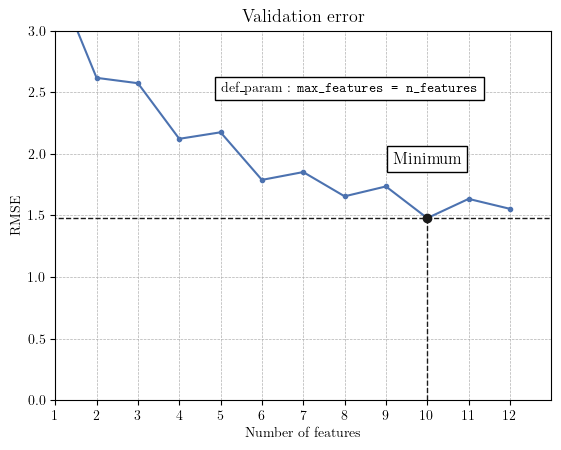
\includegraphics[width=\textwidth]{02_figures/featureserrro.png}
%     % \end{figure}
%     \captionof{figure}{Effects of number of features on RMSE}
%     \label{fig:featureserror}
% \end{minipage}%
% \begin{minipage}[t]{.5\textwidth}
%     \centering
%     % \begin{figure}
%     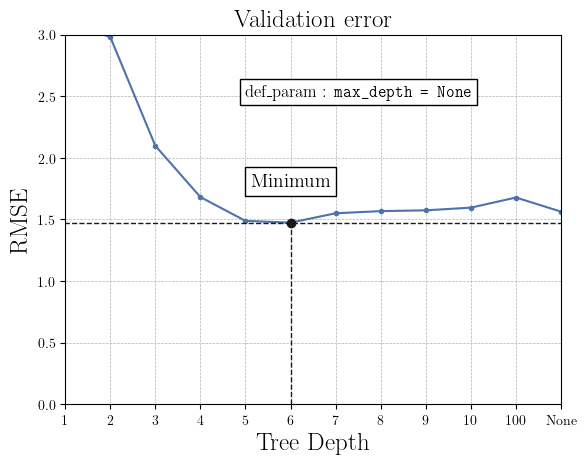
\includegraphics[width=\textwidth]{02_figures/depthError.png}
%     % \end{figure}
%     \captionof{figure}{Effects of tree depth on RMSE}
%     \label{fig:deptherror}
% \end{minipage}
% \end{figure}

% \begin{figure}[h]
%     \centering
%         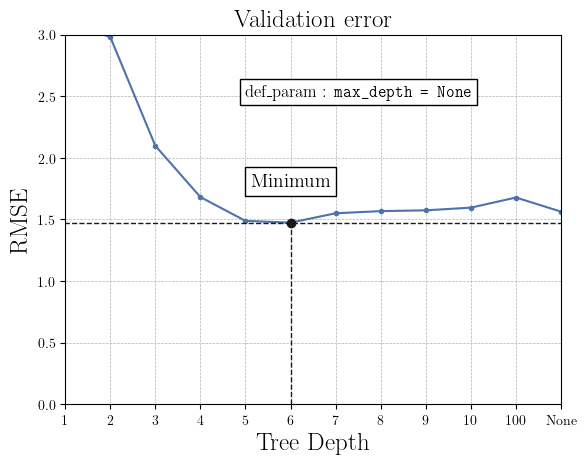
\includegraphics[width=.5\textwidth]{02_figures/depthError.png}
%         \caption{Effect of tree depth on RMSE for validation dataset}
%         \label{fig:Tree Depth Error}
% \end{figure}

% \begin{enumerate}
%     \item Possible thresholds are determined by calculating the splitting value (For example, suppose there are data points at $X = [0.2,0.4]$, then the splitting value is the value in between i.e. $t_k = 0.3$)
%     \item Calculate the mean of data points of the left and right partition space respectively, Defined by the following equation $\hat{y}_{node} = \frac{1}{m_{node}}\sum\limits_{i\in node} y ^ {(i)}$
%     \item Calculate the mean squared error (MSE) of each data points in its respective partition space. Through the equation $MSE_{node} = \sum\limits_{i\in node}(\hat{y}_{node} - y^{(i)} )^2$ 
%     \item The MSE from the respective partition space is summed.
%     \item Step $1 - 4$ is recursively repeated, until the minimum of the cost function $J(X,T_k)$, i.e. minimum MSE, is determined:
%      \begin{equation}\label{costfun}
%         J(X,t_k) = \frac{m_{left}}{m}MSE_{left} + \frac{m_{right}}{m}MSE_{right}
%         \begin{cases}
%             MSE_{node} = \sum\limits_{i\in node}(\hat{y}_{node} - y^{(i)} )^2 \\
%             \hat{y}_{node} = \frac{1}{m_{node}}\sum\limits_{i\in node} y ^ {(i)}
%         \end{cases}   
%     \end{equation}
% \end{enumerate} 